\documentclass{article}
\usepackage{ae,aecompl}
\usepackage{todonotes}
\usepackage{chngcntr}
\usepackage{tikz-cd}
\usepackage{graphicx}
\graphicspath{ {./images/}}
\usepackage[all,cmtip]{xy}
\usepackage{amsmath, amscd}
\usepackage{amsthm}
\usepackage{amssymb}
\usepackage{amsfonts}
\usepackage{bm}
\usepackage{qsymbols}
\usepackage{latexsym}
\usepackage{mathrsfs}
\usepackage{mathtools}
\usepackage{cite}
\usepackage{color}
\usepackage{url}
\usepackage{enumerate}
\usepackage{verbatim}
\usepackage[draft=false, colorlinks=true]{hyperref}
\usepackage{pdfpages}
\usepackage[margin=1.2in]{geometry}
\usepackage{IEEEtrantools}

\usepackage{fancyhdr}


\usepackage[nameinlink]{cleveref}


\DeclareMathOperator*{\ac}{accept}
\DeclareMathOperator*{\amax}{argmax}
\DeclareMathOperator*{\amin}{argmin}
\DeclareMathOperator*{\Aut}{Aut}
\newcommand {\al}{{\alpha}}
\newcommand {\abs}[1]{{\left\lvert#1\right\rvert}}
\newcommand {\A}{{\mathcal{A}}}
\newcommand {\AM}{{\mathrm{AM}}}
\newcommand {\AMp}{{\AM_{p}^{X}\!(\Ri_\w)}}
\newcommand {\B}{{\mathcal{B}}}
\DeclareMathOperator*{\Be}{Bern}
\newcommand {\Br}{{\dot{B}}}
\newcommand {\Ba}{{\mathfrak{B}}}
\newcommand {\C}{{\mathbb C}}
\newcommand {\ce}{\mathrm{c}}
\newcommand {\Ce}{\mathrm{C}}
\newcommand {\Cc}{\mathrm{C_{c}}}
\newcommand {\Ccinf}{\mathrm{C_{c}^{\infty}}}
\DeclareMathOperator{\cov}{Cov}
\DeclareMathOperator{\DEV}{DEV}
\newcommand {\Di}{{\mathbb D}}
\newcommand {\dom}{\mathrm{dom}}
\newcommand{\dist}{\stackrel{\mathrm{dist}}{=}}
\newcommand {\ud}{\mathrm{d}}
\newcommand {\ue}{\mathrm{e}}
\newcommand {\eps}{\varepsilon}
\newcommand {\veps}{\varepsilon}
\newcommand {\vrho}{{\varrho}}
\newcommand {\E}{{\mathbb{E}}}
\newcommand {\Ec}{{\mathcal{E}}}
\newcommand {\Ell}{L}
\newcommand {\Ellp}{{L_{p}[0,1]}}
\newcommand {\Ellpprime}{{L_{p'}([0,1])}}
\newcommand {\Ellq}{{L_{q}([0,1])}}
\newcommand {\Ellqprime}{{L_{q'}([0,1])}}
\newcommand {\Ellr}{L^{r}}
\newcommand {\Ellone}{{L_{1}([0,1])}}
\newcommand{\Elltwo}{{L_{2}([0,1])}}
\newcommand{\Ellinfty}{L^{\infty}}
\newcommand{\Ellinftyc}{L_{\mathrm{c}}^{\infty}}
\newcommand{\exb}[1]{\exp\left\{#1\right\}}
\DeclareMathOperator*{\Ext}{Ext}
\newcommand{\F}{{\mathcal{F}}}
\newcommand{\Fe}{{\mathbb{F}}}
\newcommand{\G}{{\mathcal{G}}}
\newcommand{\HF}{\mathcal{H}_{\text{FIO}}^{1}(\Rd)}
\newcommand{\Hr}{H}
\newcommand{\HT}{\mathcal{H}}
\newcommand{\ui}{\mathrm{i}}
\newcommand{\I}{{I}}
\newcommand{\J}{{\mathcal{J}}}
\newcommand{\id}{{\mathrm{id}}}
\newcommand{\iid}{\stackrel{\mathclap{\normalfont\mbox{iid}}}{\sim}}
\newcommand{\im}{{\text{im }}}
\newcommand{\ind}{{\perp\!\!\!\perp}}
\DeclareMathOperator*{\Int}{int}
\newcommand{\intx}{{\overline{\int_{X}}}}
\newcommand{\inte}{{\overline{\int_{\E}}}}
\newcommand{\la}{\lambda}
\newcommand{\rb}{\rangle}
\newcommand{\lb}{{\langle}}
\newcommand{\La}{\Lambda}
\newcommand{\calL}{{\mathcal{L}}}
\newcommand{\lp}{{\mathcal{L}}^{p}}
\newcommand{\lpo}{{\overline{\mathcal{L}}^{p}\!}}
\newcommand{\Lpo}{{\overline{\Ell}^{p}\!}}
\newcommand{\M}{{\mathbf{M}}}
\newcommand{\Ma}{{\mathcal{M}}}
\newcommand{\N}{{{\mathbb N}}}
\newcommand{\Na}{{{\mathcal{N}}}}
\newcommand{\norm}[1]{\left\|#1\right\|}
\newcommand{\normm}[1]{{\left\vert\kern-0.25ex\left\vert\kern-0.25ex\left\vert #1 
    \right\vert\kern-0.25ex\right\vert\kern-0.25ex\right\vert}}
\newcommand{\Om}{{{\Omega}}}
\newcommand{\one}{{{\bf 1}}}
\newcommand{\pic}{\text{Pic }}
\newcommand{\ph}{{\varphi}}
\newcommand{\Pa}{{\mathbb{P}}}
\newcommand{\Po}{{\mathcal{P}}}
\newcommand{\Q}{{\mathbb{Q}}}
\newcommand{\R}{{\mathbb R}}
\newcommand{\Rd}{{\mathbb{R}^{d}}}
\DeclareMathOperator{\rej}{reject }
\newcommand{\Rn}{{\mathbb{R}^{n}}}
\newcommand{\cR}{{\mathcal{R}}}
\newcommand{\Rad}{{\mathrm{Rad}}}
\newcommand{\ran}{{\mathrm{ran}}}
\newcommand{\Ri}{{\mathrm{R}}}
\newcommand{\supp}{{\mathrm{supp}}}
\newcommand{\Se}{\mathrm{S}}
\newcommand{\Sp}{S^{*}(\Rn)}
\newcommand{\St}{{\mathrm{St}}}
\newcommand{\Sw}{\mathcal{S}}
\newcommand{\T}{{\mathcal{T}}}
\newcommand{\ta}{{\theta}}
\newcommand{\Ta}{{\Theta}}
\newcommand{\topp}{\stackrel{p}{\to}}
\newcommand{\todd}{\stackrel{d}{\to}}
\newcommand{\toL}[1]{\stackrel{L^{#1}}{\to}} 
\newcommand{\toas}{\stackrel{a.s.}{\to}}
\DeclareMathOperator{\V}{Var}
\newcommand {\w}{{\omega}}
\newcommand {\W}{{\mathrm{W}}}
\newcommand {\Wnp}{\text{$\mathrm{W}$\textsuperscript{$n,\!p$}}}
\newcommand {\Wnpeq}{\text{$\mathrm{W}$\textsuperscript{$n\!,\!p$}}}
\newcommand {\Wonep}{\text{$\mathrm{W}$\textsuperscript{$1,\!p$}}}
\newcommand {\Wonepeq}{\text{$\mathrm{W}$\textsuperscript{$1\!,\!p$}}}
\newcommand {\X}{{\mathcal{X}}}
\newcommand {\Z}{{{\mathbb Z}}}
\newcommand {\Za}{{\mathcal{Z}}}
\newcommand {\Zd}{{\Z[\sqrt{d}]}}
\newcommand {\vanish}[1]{\relax}

\newcommand {\wh}{\widehat}
\newcommand {\wt}{\widetilde}
\newcommand {\red}{\color{red}}

% Distributions
\newcommand{\normal}{\mathsf{N}}
\newcommand{\poi}{\mathsf{Poisson}}
\newcommand{\bern}{\mathsf{Bernoulli}}
\newcommand{\bin}{\mathsf{Binomal}}
\newcommand{\multi}{\mathsf{Multinomial}}
\newcommand{\Exp}{\mathsf{Exp}}



% put your command and environment definitions here




% some theorem environments
% remove "[theorem]" if you do not want them to use the same number sequence


  \newtheorem{thrm}{Theorem}
  \newtheorem{lemma}{Lemma}
  \newtheorem{prop}{Proposition}
  \newtheorem{cor}{Corollary}

  \newtheorem{conj}{Conjecture}
  \renewcommand{\theconj}{\Alph{conj}}  % numbered A, B, C etc

  \theoremstyle{definition}
  \newtheorem{defn}{Definition}
  \newtheorem{ex}{Example}
  \newtheorem{exs}{Examples}
  \newtheorem{question}{Question}
  \newtheorem{remark}{Remark}
  \newtheorem{notn}{Notation}
  \newtheorem{exer}{Exercise}


\newcommand{\pc}{{\text{pcr}(k)}}
\newcommand{\rhat}{\wh{\text{Risk}}}

\title{STATS305A - Lecture 14}
\author{John Duchi\\ Scribed by Michael Howes}
\date{11/09/21}

\pagestyle{fancy}
\fancyhf{}
\rhead{STATS305A - Lecture 14}
\lhead{11/09/21}
\rfoot{Page \thepage}

\begin{document}
\maketitle
\tableofcontents
\section{Announcements}
\begin{itemize}
    \item HW 3 out now.
    \item An etude coming soon.
    \item There will be four homeworks and four etudes in total for the course.
\end{itemize}
\section{Recap}
\subsection{Ridge regression}
Last time, we started to discuss ridge regression. In ridge regression we use the estimator
\[\wh{\beta}_\la = \amin_\la \left\{\norm{Xb-Y}_2^2+\la\norm{b}_2^2\right\}. \]
We saw that if $U\Gamma V^T$ is the SVD of $X$, then we have 
\begin{align*}
    H_\la &:= X(X^TX+\la I)^{-1}X^T\\
    &= U\diag\left(\frac{\gamma_j^2}{\gamma_j^2+\la}\right)U^T,
\end{align*}
and our predictions are given by
\[\wh{Y}_\la = H_\la Y = \sum_{j=1}^d \frac{\gamma_j^2}{\gamma_j^2+\la}u_ju_j^TY. \]
We also saw that when doing ridge regression we often replace $Y$ with $Y-\bar{Y}\one$.
\subsection{PCA}
We also started talking about principal component analysis (PCA). We wanted to project each $x_i \in \R^d$ onto the directions in $\R^d$ capturing the most variance in our data $X$. Equivalently we want to project onto the subspace closest to all the $x_i's$. 
\section{Principal component regression}
Roughly, if $y$ is related to $x$ we'd hope that the variance in $y$ is explained by the most varying/important direction in $X$. 

Recall that if $X = U\Gamma V^T$ is the SVD of $X$, then the first $k$ principal components are the first $k$ vectors in $V = [v_1,v_2,\ldots, v_d]$. The idea behind principal component regression (pcr) is to replace $x_i \in \R^d$ with the projection of $x_i$ onto $\spn(V_k)$ where $V_k = [v_1,\ldots, v_k]$. Define $\wt{x}_i = V_kV_k^T x_i$. We will then run regression on 
\[\wt{X} = \begin{bmatrix}
    \wt{x}_1^T\\ \vdots \\ \wt{x}_n^T
\end{bmatrix} \in \R^{n \times d}. \]
Thus our estimate of $\beta$ is
\[\wh{\beta}_{\pc} = \amin_b \norm{Y-\wt{X}b}_2^2. \]
We can formulate this as doing regression in $\R^k$. Note that $\wt{X}=XV_kV_k^T$ thus we can let $c = V_k^Tb \in \R^k$ so that $\wt{X}b = XV_k c$. We can this instead solve
\[\wh{c} = \amin_{c \in \R^k} \norm{Y-XV_k c} = \amin_{c \in \R^k}\norm{Y-U\Gamma V^TV_k c}. \]
Note that 
\[V^TV_k = \begin{bmatrix}
    I_k \\ 0
\end{bmatrix}, \]
and so
\[\wh{c} = \amin_{c \in \R^k}\norm{Y-U\Gamma V^TV_k c} = \amin_{c\in \R^k} \norm{Y-U_k \Gamma_k c},\]
where $U_k = [u_1,\ldots, u_k] \in \R^{n \times k}$ and $\Gamma_k = \diag(\gamma_1,\ldots, \gamma_k)$. Thus 
\[\wh{c} = \Gamma_k^{-1}U_k^T Y, \]
and 
\[\wh{\beta}_\pc =  V_k \Gamma_k^{-1} U_k Y.\]
Thus in PCR we project $X$ onto the span of the first $k$ left singular vector $X$ and then fit $Y$ as well as possible within that span. The predictions from PCR are thus 
\begin{align*}
    \wh{Y}_\pc &= X\wh{\beta}_\pc \\
    &=U\Gamma V^T V_k \Gamma^{-1} U_k^T Y\\
    &= U_k U_k^T Y\\
    &= H_k Y.
\end{align*}
Thus 
\[\wh{Y}_\pc = H_k Y = \sum_{j=1}^k u_ju_j^TY.\] 
We can compare this to ridge regression 
\[\wh{Y}_\la = \sum_{j=1}^d \frac{\gamma_j^2}{\gamma_j^2+\la} u_ju_j^T Y. \]
In ridge regression we apply a soft threshold to each of the singular direction $u_j$ where we shrink by the factor $\frac{\gamma_j^2}{\gamma_j^2+\la}$ which increases with $j$. In PCR we have a hard threshold where we cut off the singular directions $u_j$ for $j > k$. The thresholds look something like this:

\begin{center}
    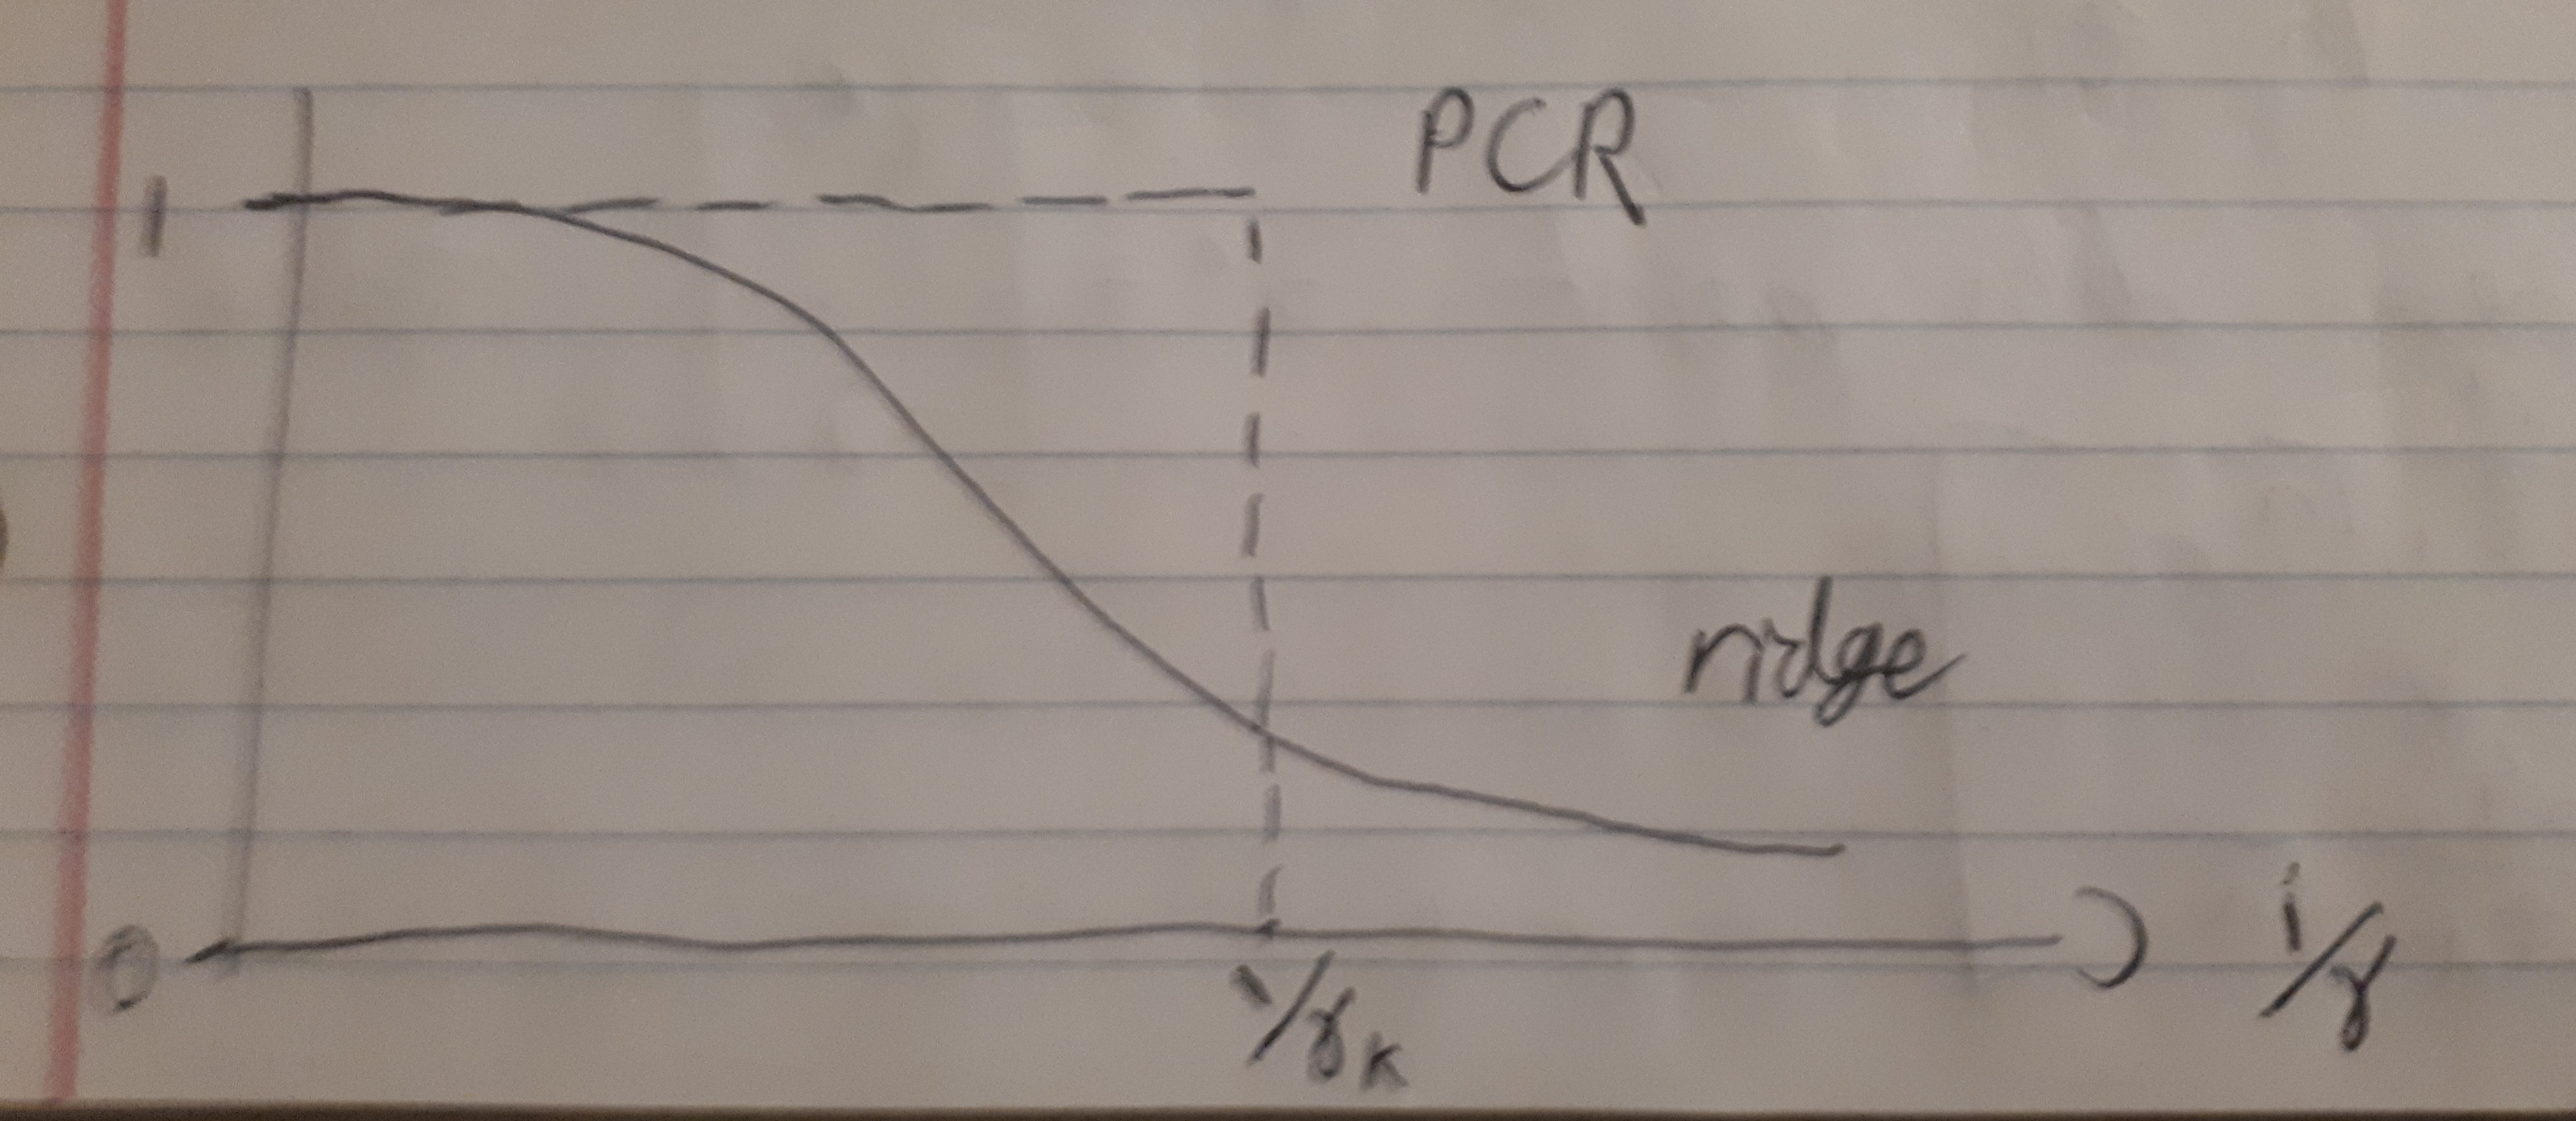
\includegraphics[width = \textwidth/2]{11_09_P01.jpg}
\end{center}

\begin{remark}
    A good question from the audience: what about the scale of the columns in 
    \[X = [x^{(1)},\ldots, x^{(d)}]?\] 
    In  PCR we always standardize data so that $\E[x^{(j)}]=0$ and $\V(x^{(j)})=0$. This is to avoid situations like this 

    \begin{center}
        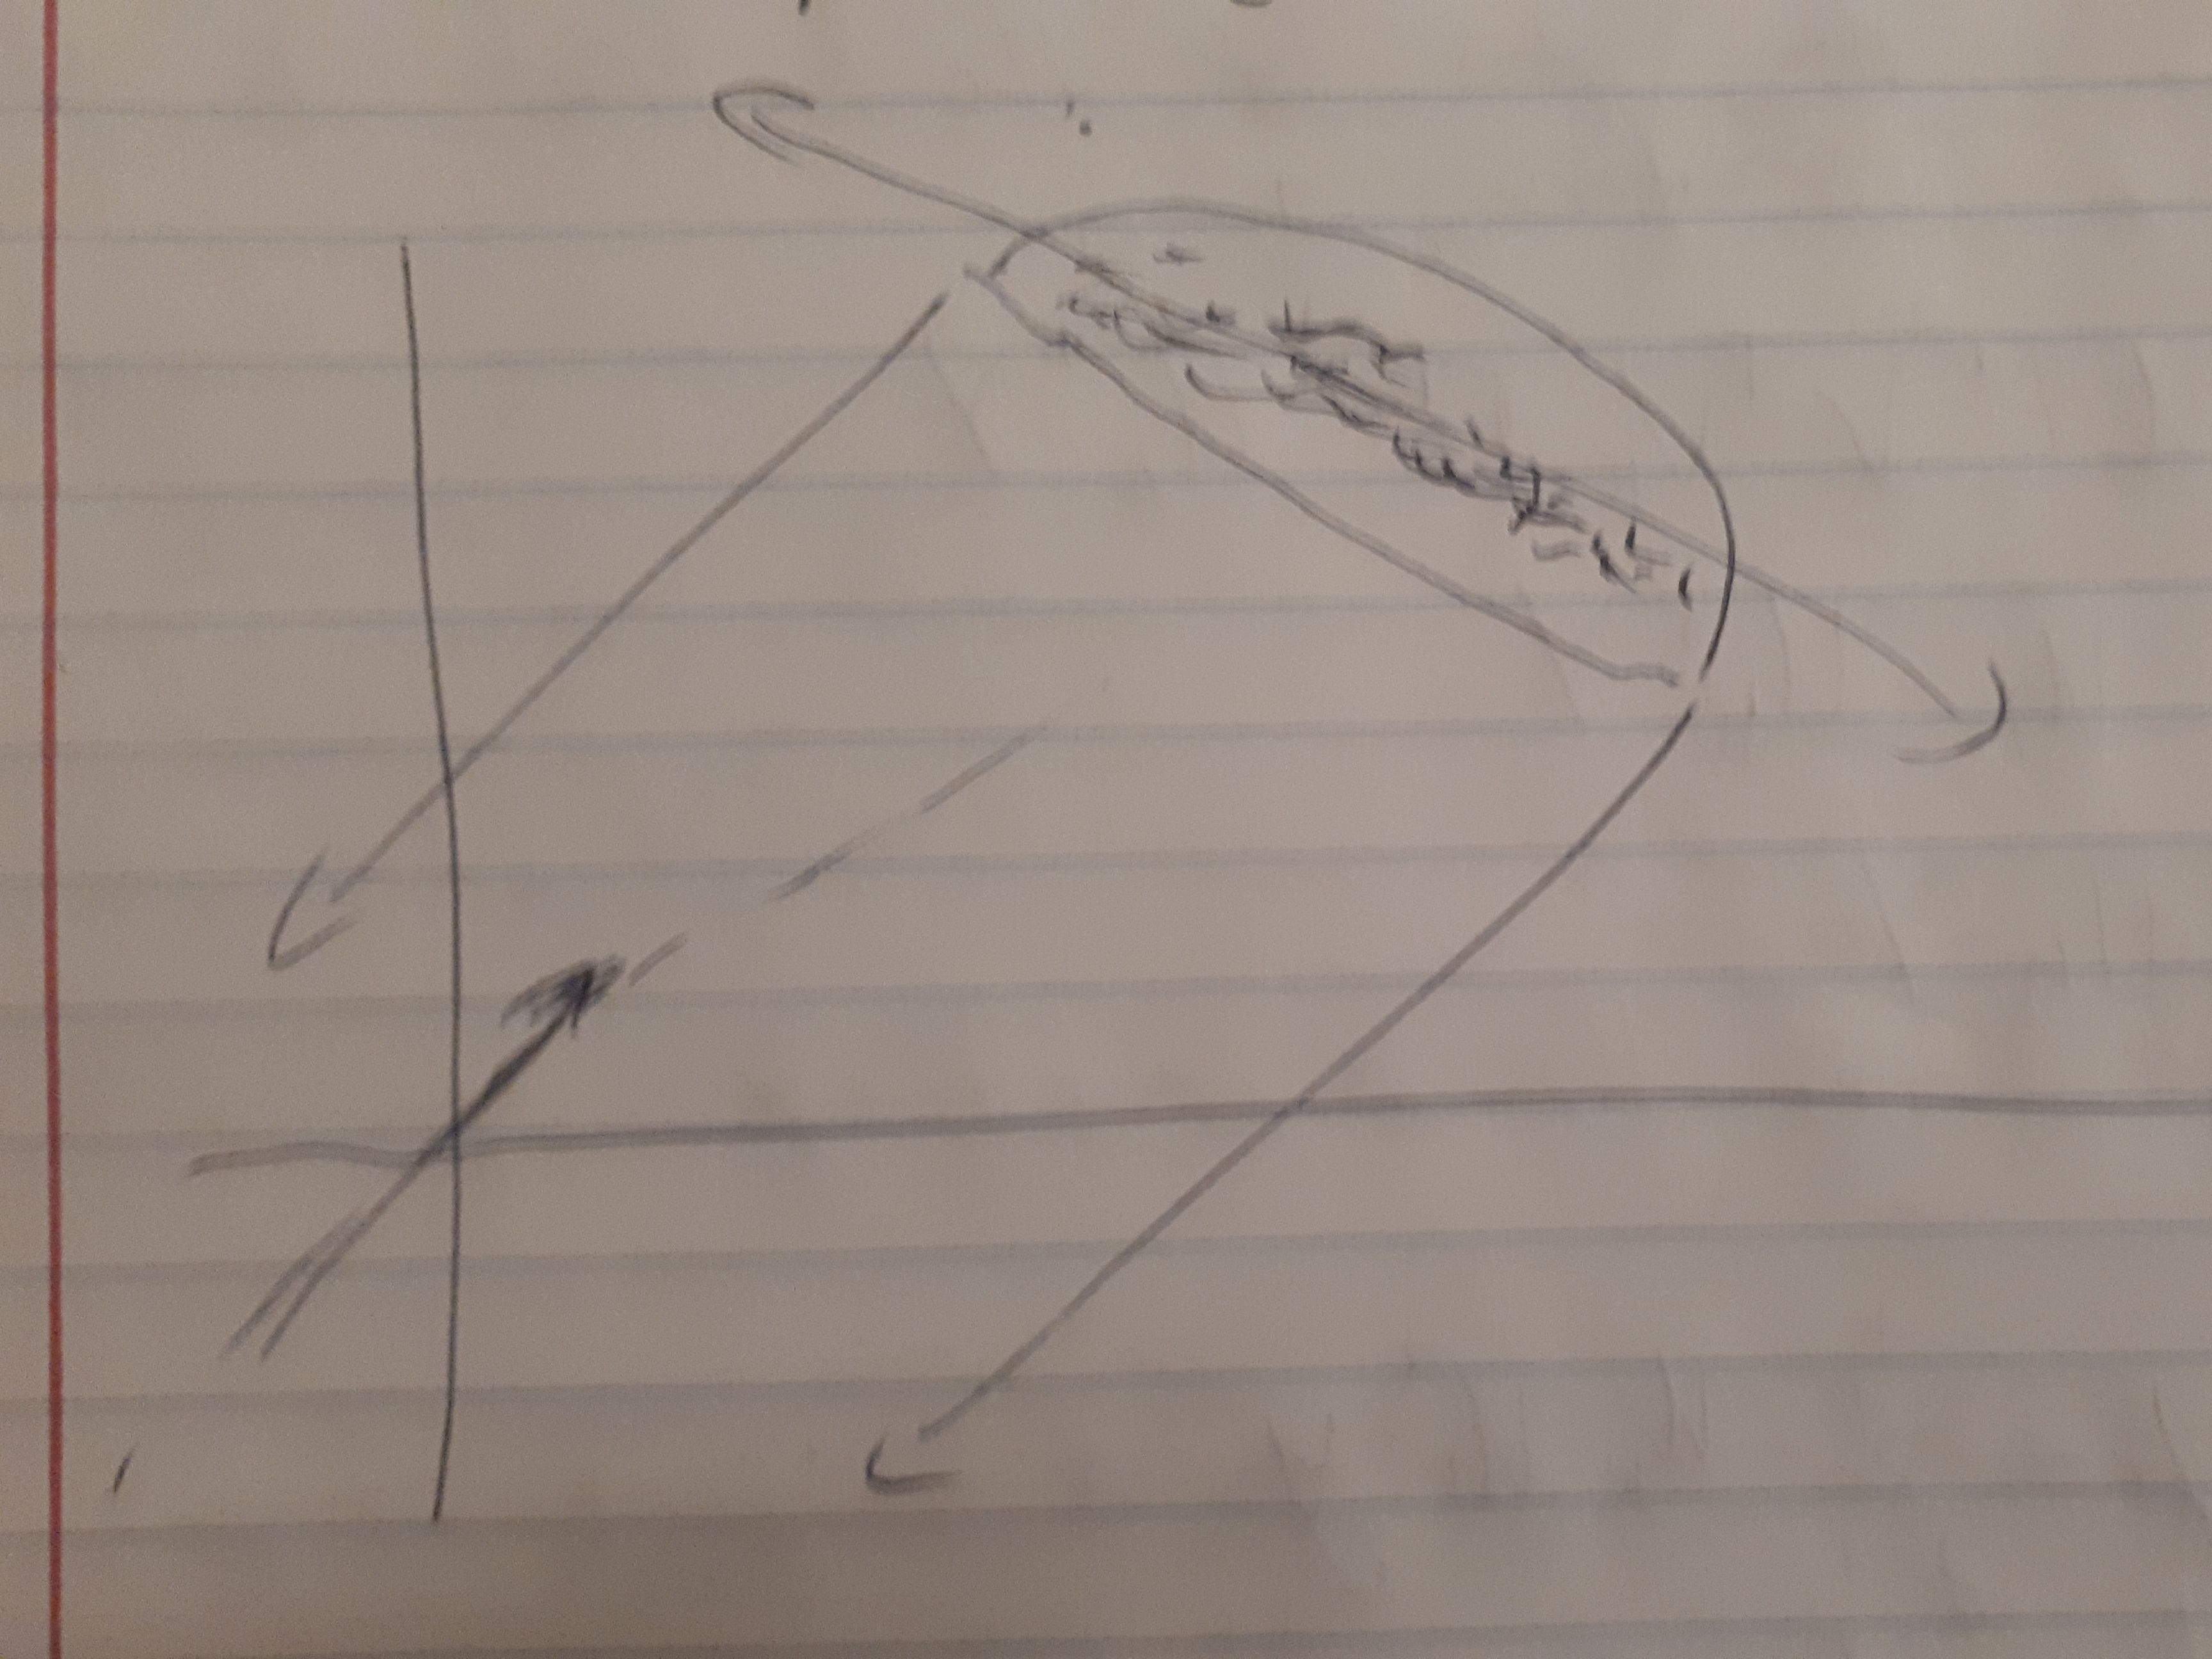
\includegraphics[width = \textwidth/2]{11_09_P02.jpg}   
    \end{center}

    To do this we set $\wh{\tau}_j^2 = \norm{x^{(j)}}_2^2$. and replace $x^{(j)}$ with $\sqrt{n} \frac{x^{(j)}}{\wh{\tau}_j}$. If we see a new data point $x^*=[x_1^*,\ldots, x_d^*]^T$, to make predictions we have to first perform the transformation
    \[x^* \mapsto \begin{bmatrix}
        \sqrt{n} \frac{x_1^*}{\wh{\tau}_1}\\ \vdots \\ \sqrt{n} \frac{x_d^*}{\wh{\tau}_d}
    \end{bmatrix}.\]
    But sometimes we care about the scale of the variables and wouldn't want to standardize. This is a problem specific issue that can be hard. Boosting is a technique we will see later that can help. Boosting allows this process to be automized.
\end{remark}
\begin{remark}
    On the homework we are asked to compute the optimism/bias in PCR and ridge regressions. That is, what are the effective degrees of freedom in PCR and ridge?
\end{remark}
\section{Feature selection methods}
Given $X = [x^{(1)},\ldots, x^{(d)}] \in \R^{n \times d}$, which features should we include? That is, which columns of $X$ should we include in our regression?

A common approach is to pick different index subsets $J \subseteq [d] = \{1,\ldots, d\}$. We then fit a model on $X_j = [x^{(j)}]_{j \in J} \in \R^{n \times \abs{J}}$. We then ask if the fitted model is ``good enough''. Our goal is to choose $J$ to minimize erros on future data. There are two approaches for evaluating which subsets are ``good enough''
\begin{itemize}
    \item Hold out some data in a test set $(x^{\text{test}}, y^{\text{test}})$ and evaluate the model on this test set. We will talk about this and variations such as permutation tests and cross validation in later lectures.
    \item Penalization approaches where we penalize the complexity of $J$ using something like Mallows's $C_p$ statistic.
\end{itemize}
The notation we will use is
\[\rhat(\beta) = \text{estimated error or risk on future data}.\]
The quantity $\rhat(\beta)$ will be the basis for which we select models. For example we may have 
\[\rhat(\beta) = \frac{1}{n}\norm{X \beta - Y}_2^2 + \frac{2\wh{\sigma}^2p}{n}, \]
where $p = \norm{\beta}_0 = \#$ of non-zero entries. Or we might have
\[\rhat(\beta) = \frac{1}{n_{\text{test}}}\norm{X^\text{test}\beta - Y^{\text{test}}}_2^2. \]
\subsection{All subsets}
In all subsets regression, we do the following:
\begin{itemize}
    \item Lookkat all subsets $J \subseteq [d]$.
    \item Compute $\wh{\beta}_J = \amin_b \norm{X_J b- Y}_2^2$.
    \item Choose $\wh{\beta}$ to be the minimizer of $\rhat(\wh{\beta}_J)$.
\end{itemize}
There are some challenges to all subset regression.
\begin{itemize}
    \item There are $2^d$ such subsets which means it can very expensive. (In practice, branch and bound methods can allow $d \sim 1000$).
    \item Often the results are optimiistic. Since we are searching over \emph{so} many possible models, the models might overfit even with a good choice of $\rhat$.
    \item The effictiveness of methods (especially when compared to convex optimization based approaches like ridge regression) depends \emph{a lot} on $\sigma^2 = \V(y|x)$. If 
    \[ \frac{\V(x^T\beta)}{\sigma^2},\]
    is large (most of the variance is explained by $x$), then all subsets is good. Otherwise all subsets is not so good.
    \item Recommended reading: \href{https://projecteuclid.org/journals/statistical-science/volume-35/issue-4}{this issue of Statistical Science} on all subsets regression. See in particular the parts written by
    \begin{itemize}
        \item Bertsimas,
        \item Mazumdar,
        \item Hastie/Tibshirani/Tibshirani.
    \end{itemize}
\end{itemize}
\subsection{Forward stepwise}
Consider the following greedy algorithm.
\begin{itemize}
    \item Pick the feature $j$ not in the model that makes the most progress. Add feature $j$ to the model.
    \item Repeat.
\end{itemize}
For formally, Set $J=\emptyset$. Then for $p=1,2,\ldots$:
\begin{itemize}
    \item Define $J_{+j}= J \cup \{j\}$ and $r_j^2 = \min_b \norm{X_{J+j}b - y}_2^2$ for $j \notin J$.
    \item Set $j^* = \amin_j r_j^2$.
    \item Update $J$ to $J\cup \{j^*\}$. 
\end{itemize}
This is a reasonable approach and can be computed quickly. It is often effective even when $d$ is large. The idea is that we would run this until the improvements get small. The plot of the residuals against $\abs{J}$ would look something like this:

\begin{center}
    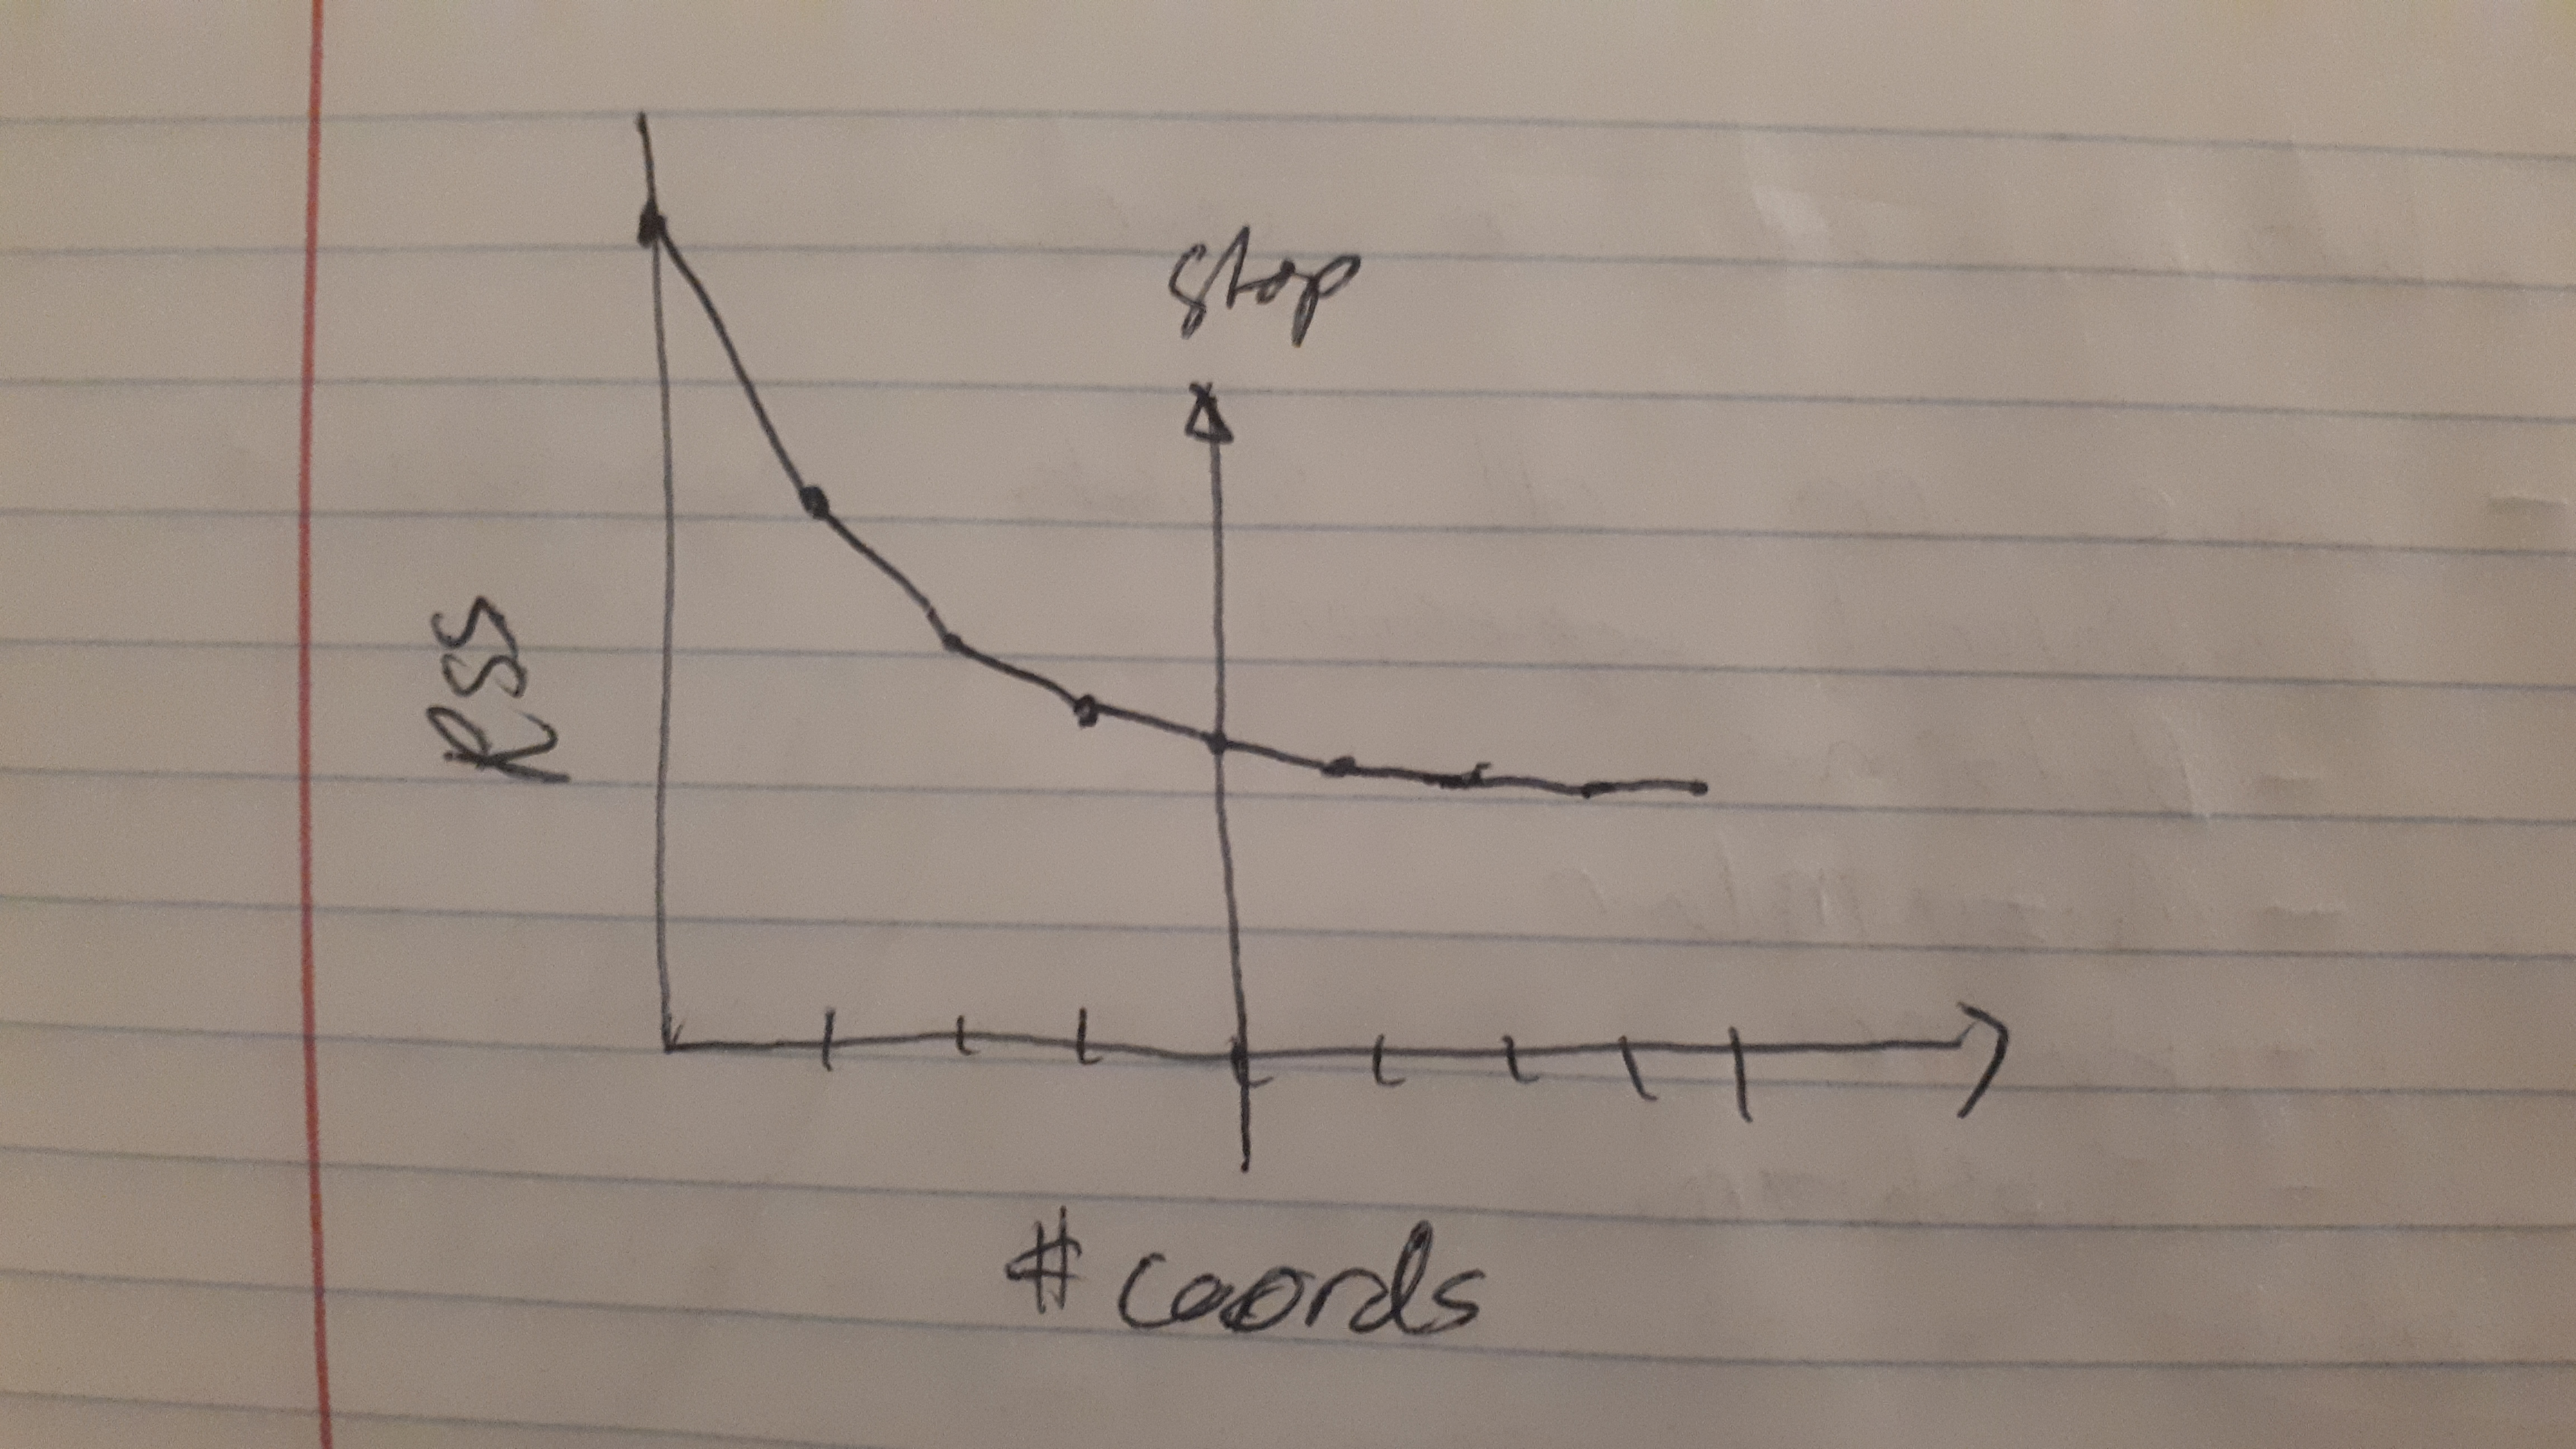
\includegraphics[width = \textwidth/2]{11_09_P03.jpg}
\end{center}

When doing the forward stepwise algorithm we will need to make approximate $d^2 << 2^d$ computations of $r_j^2$. Thus it is much better than a naive implementation of all subsets. 

\subsection{Backwards stepwise}
Unfortunately the forward stepwise algorithm is a greedy algorithm and we might end up with some junk. This gives us the backwards stepwise algorithm. 
\begin{itemize}
    \item First fit using the full model (or the model produced by the forwards stepwise algorithm).
    \item Iteratively remove coordinates that increase $RSS$ the least.
\end{itemize}
\section{Boosting}
This techinique was originally developed in 1995 by Freund and Schapire in work on clustering. 

It is designed to solve the challenge that we often do not know any of the following:
\begin{itemize}
    \item What scales to use.
    \item What non-linear transformation to use.
\end{itemize}
Suppose we have a tool that can fit a small model well (a weak-learner). We then have the procedure:
\begin{itemize}
    \item Start with raw data $(x,y) \in \X \times \R$.
    \item Iteratively\begin{itemize}
        \item Find some feature mapping $\phi : \X \to \R$ capturing some signal in $x$ about $y$.
        \item Add this feature to the model we're building.
    \end{itemize}
\end{itemize}
More formally, for $j=1,2,\ldots$, pick $\phi^{(j)} : \X \to \R$ and add $\phi^{(j)}$ to the model
\[M(X) = \begin{bmatrix}
    \phi^{(1)}(x_1)&\phi^{(2)}(x_1)&\ldots & \phi^{(j)}(x_1)\\
    \phi^{(1)}(x_2)&\phi^{(2)}(x_2)&\ldots & \phi^{(j)}(x_2)\\
    \vdots & \vdots & \ddots & \vdots \\
    \phi^{(1)}(x_n)&\phi^{(2)}(x_n)&\ldots & \phi^{(j)}(x_n) 
\end{bmatrix}\in \R^{n \times d}. \]
Fit a model and repeat. 

How do  we actually do this? Roughly: coordinate descent. We first fix a family $\Phi$ of feature mappings. For example we may use decision stumps for $x \in \R^d$
\[\phi(x) = \begin{cases}
    1 & \text{if } x_j \ge \tau,\\
    0 & \text{if } x_j < \tau.
\end{cases} \]
That is $\Phi$ consists of 0-1 thresholds on individual coordinates of raw data. The function $\phi$ looks like this

\begin{center}
    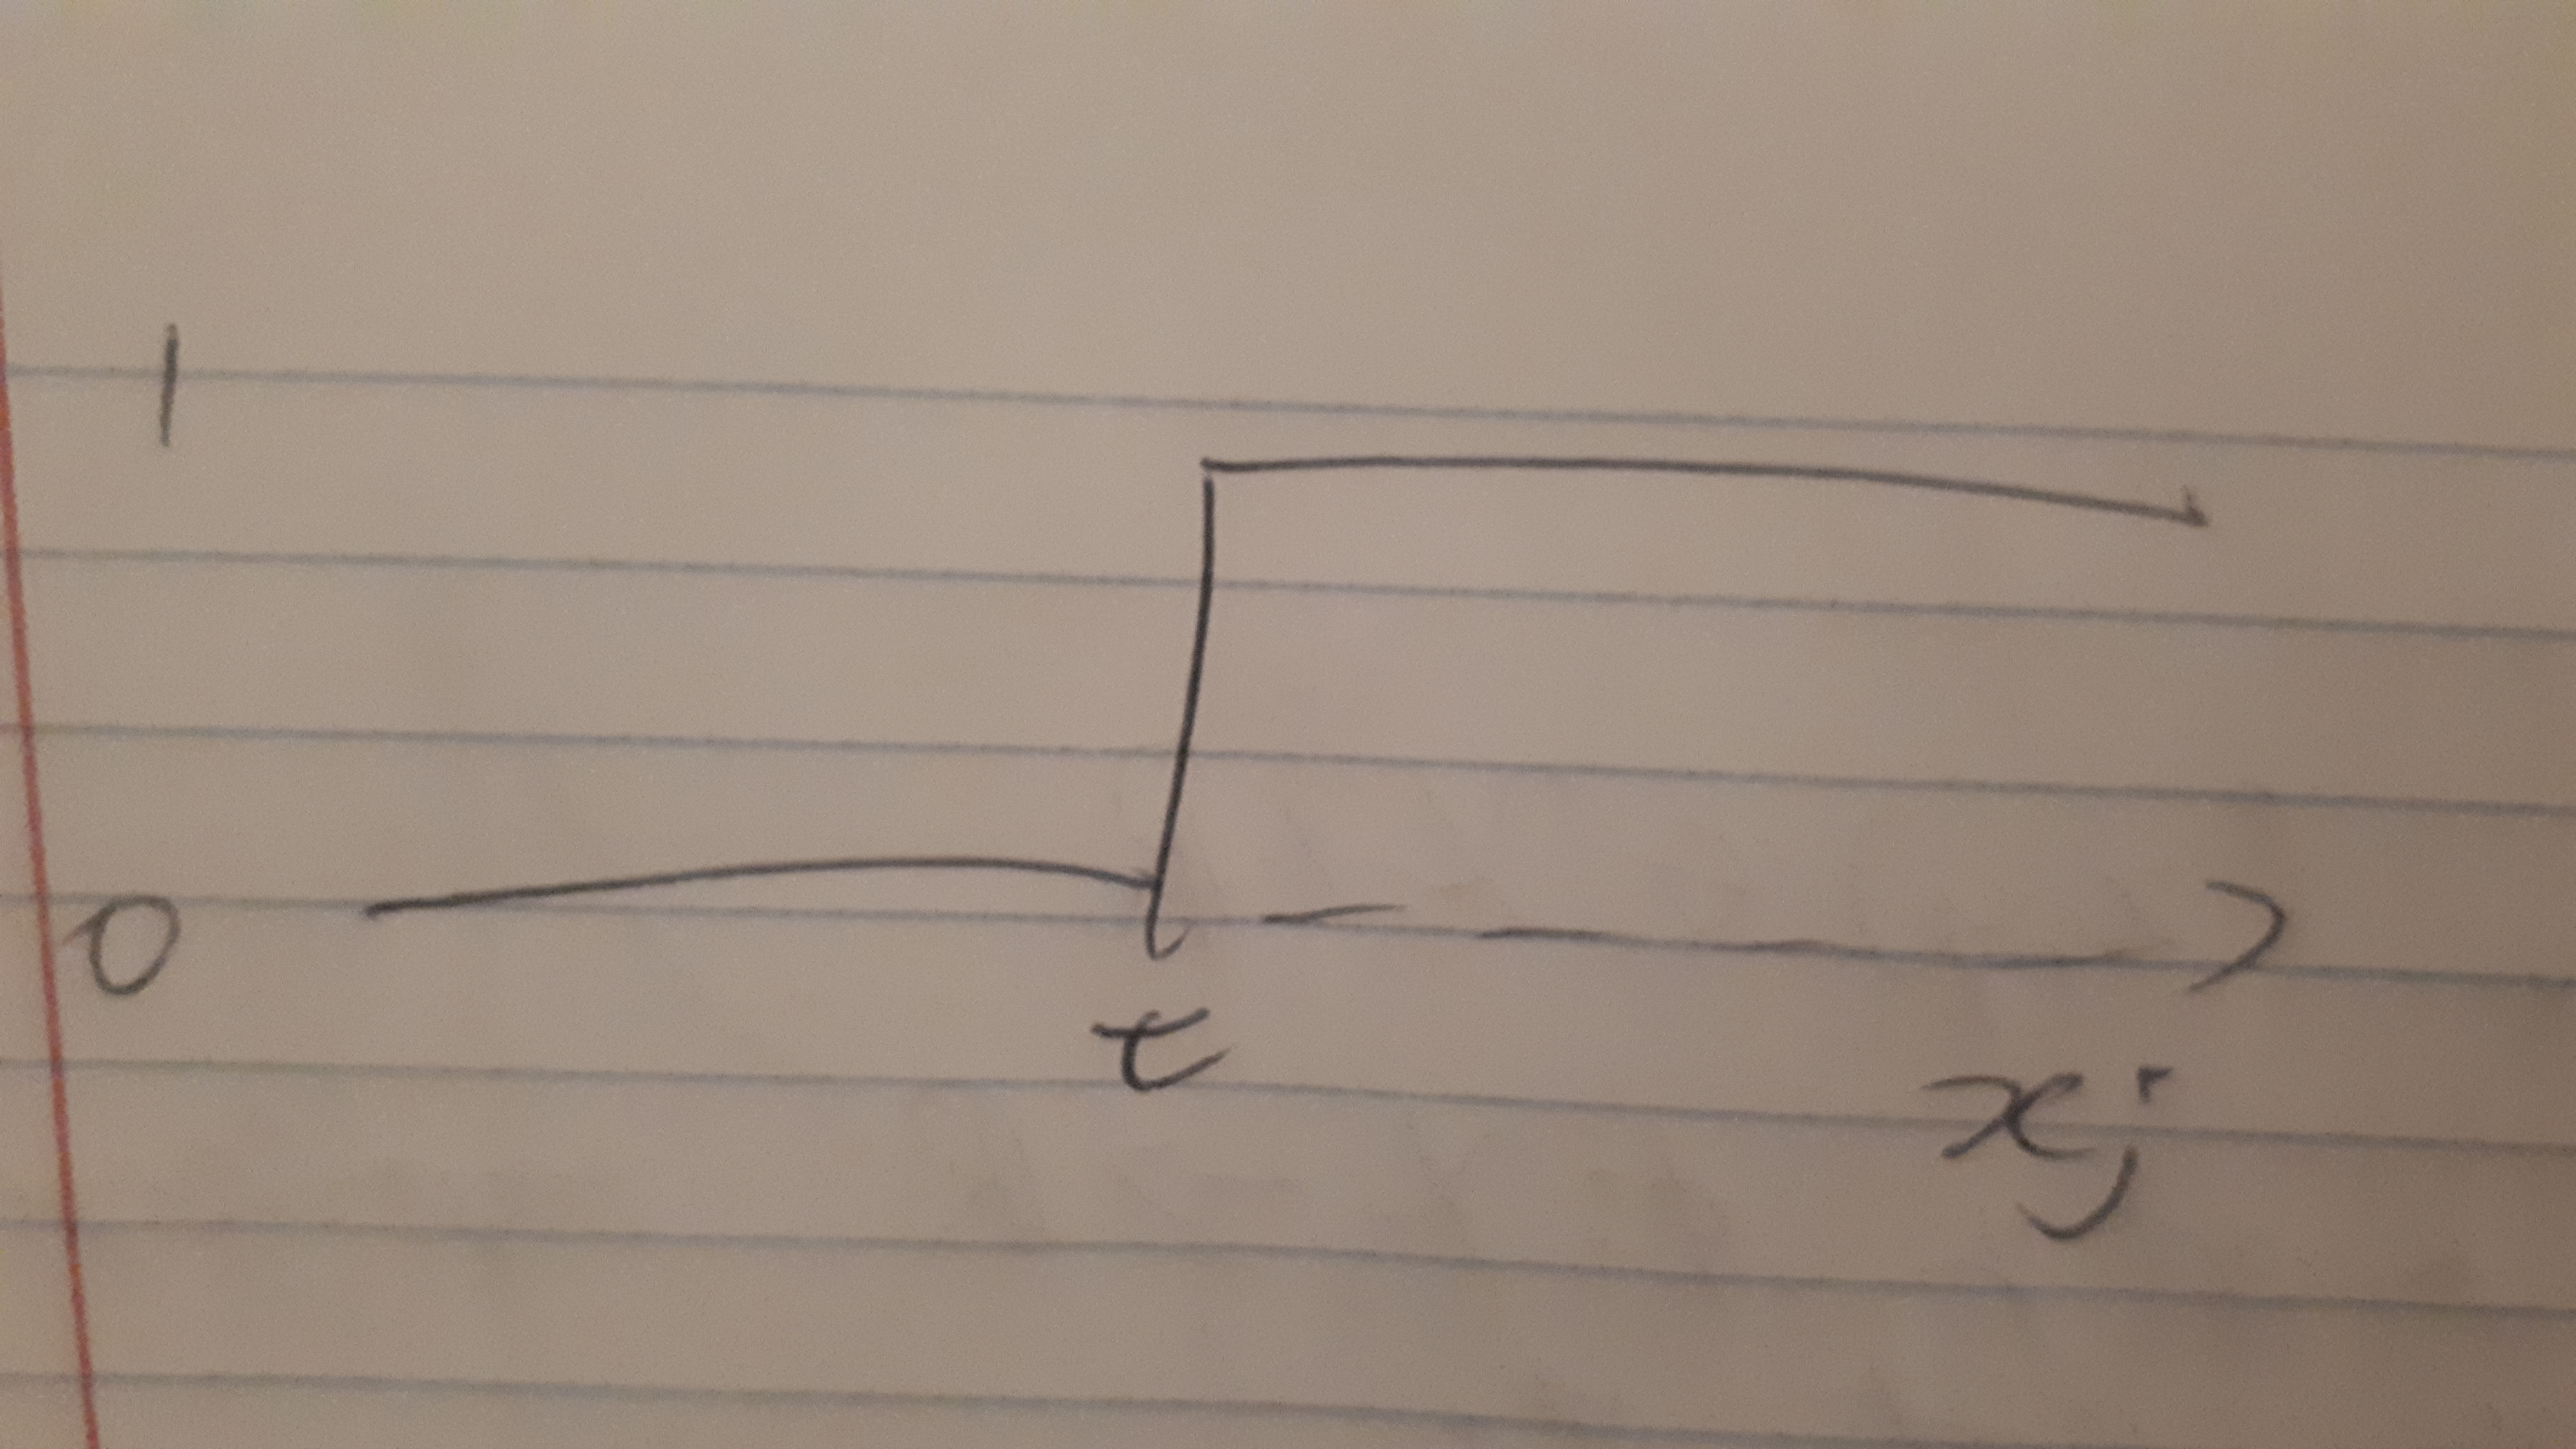
\includegraphics[width = \textwidth/2]{11_09_P04.jpg}
\end{center}

The idea is that we start with $M(X)$ and ask which feature improves the risk the most. That is we define 
\[R(\delta,\phi; M) = \norm{[M,\phi]\begin{bmatrix}\beta\\ \delta \end{bmatrix} - y}_2^2, \]
where $\beta$ is the minimizer of $\norm{Mb-y}_2^2$. There are then two approaches:
\begin{itemize}
    \item Ask for
    \[\wh{\delta} = \amin_\delta R(\delta, \phi;M).\]
    \item Or ask what gives the most local progress 
    \[R'(\delta,\phi;M)|_{\delta = 0}.\]
\end{itemize}
We will discuss this more on Thursday. 
\end{document}
